\addtocontents{toc}{\protect\contentsline{chapter}{}{}{}}

\chapter{Szenarien}
\label{[chap:szenarien]}

\section{Smartphone als Präsenzsensor (Wohnung/Haus als Ganzes)}
\emph{(von Patrick Hecker)}

\subsection{Auslöser}
\begin{itemize}
	\item Smartphone (WiFi, GPS, Funkzelle)
\end{itemize}

\subsection{Ablauf}
16:00 Uhr: Person A begibt sich nach Feierabend auf den Heimweg. Die Präsenzsensor App, welche auf dem Smartphone von Person A installiert ist, wird im Umkreis von 2 km (einstellbar) um die Wohnung aktiv und sendet eine Nachricht (über HTTP) an die zentrale Steuereinheit. Das Gateway hat nun die Information, dass sich Person A auf dem Weg zur Wohnung befindet (Stufe 1) und startet in Abhängigkeit der aktuellen Personenanzahl, die sich im Haus befindet und deren Einstufung im System (Erwachsener, Kind) ein voreingestelltes Szenario. Sobald Person A zu Hause angekommen ist und die Wohnung betritt, wird sein Smartphone erneut aktiv (ohne Benutzerinteraktion\footnote{Die Präsenzsensor App registriert beim erstmaligen Start bzw. bei der Installation ein Betriebssystem-Ereignis, welches die Änderung des Netzwerkzustandes (Android: android.net.conn.CONNECTIVITY\_CHANGE) signalisiert. Sobald dieses Ereignis eintritt, wird die App aktiv und prüft die aktuellen Verbindungsinformation (WLAN ja/nein, SSID) und sendet im Hintergrund, beim Erkennen des Heimnetzes eine Nachricht an die zentrale Steuereinheit.}), da eine Verbindung zu seinem privaten WLAN-Netz hergestellt wurde. Als Reaktion auf dieses Ereignis sendet sein Smartphone erneut eine Nachricht an die zentrale Steuereinheit und signalisiert damit die Ankunft von Person A. Solange die zentrale Steuereinheit keine neuen Informationen vom Smartphone bekommt, nimmt die zentrale Steuereinheit an, dass sich Person A in der Wohnung befindet. Diese Information wird für andere Automatisierungsmechanismen zur Verfügung gestellt, um deren Entscheidungsfindung zu unterstützen.

\subsection{Modellierung}
\begin{figure}[h!]
	\centering
	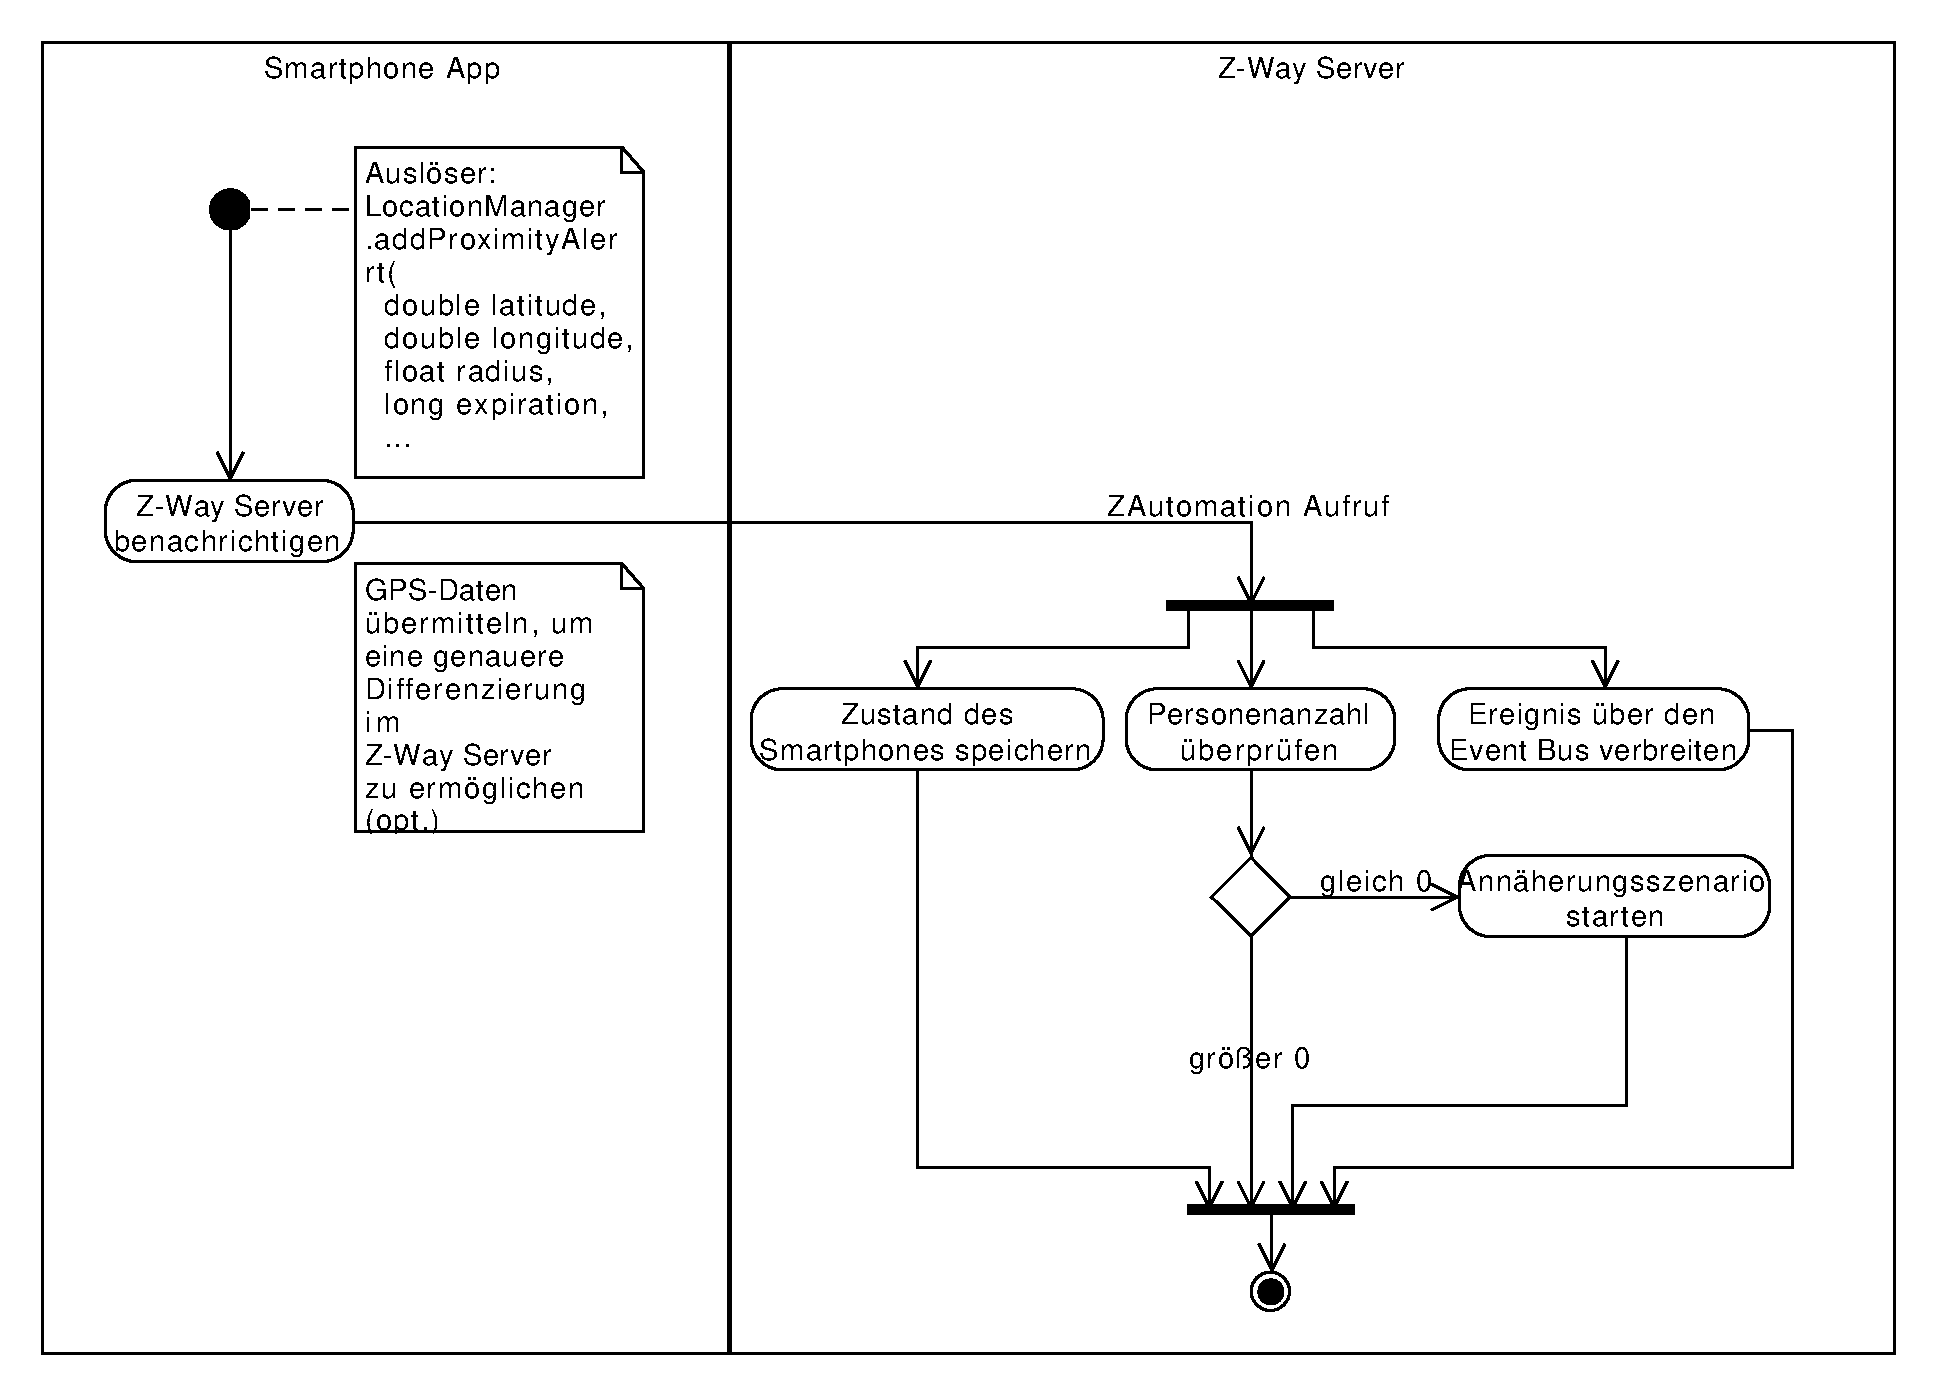
\includegraphics[width=0.9\textwidth]{img/Szenarien/SmartphoneProximity.pdf}
	\caption{Smartphone als Präsenzsensor - Modell Proximity Alert}
	\label{fig:szenarienSmartphoneProximity}
\end{figure}

\begin{figure}[h!]
	\centering
	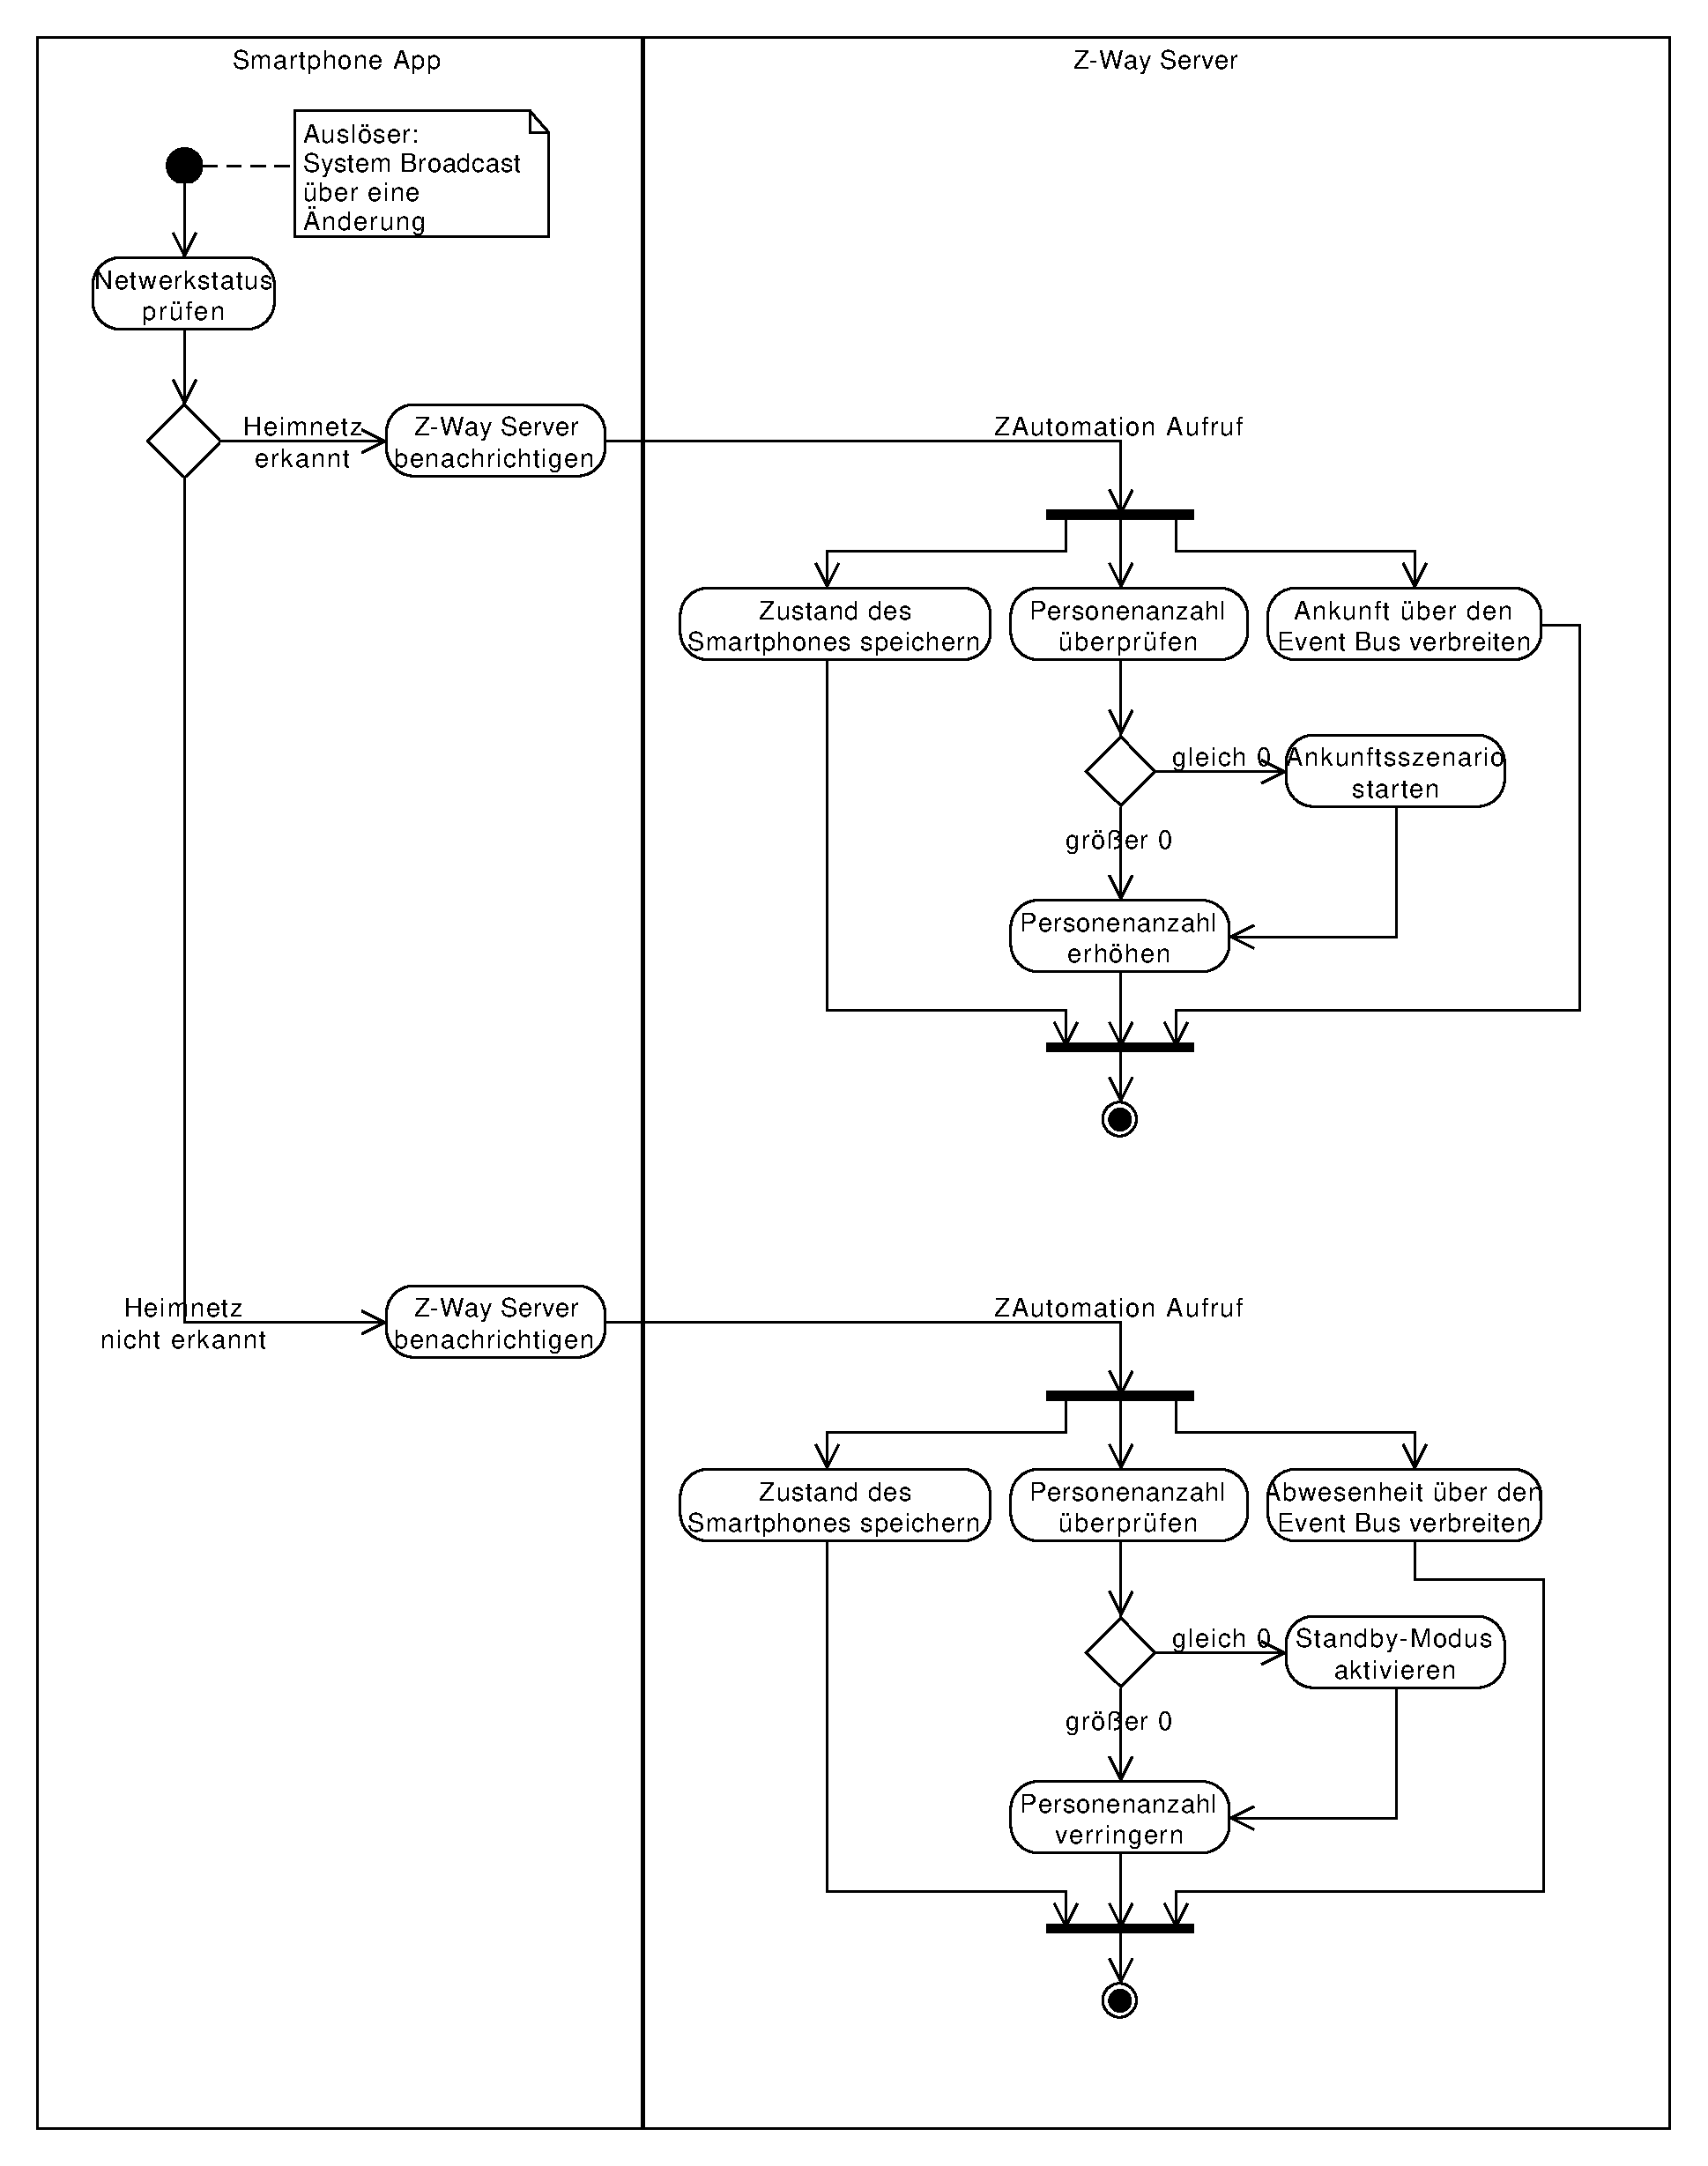
\includegraphics[width=1.0\textwidth]{img/Szenarien/SmartphoneWlan.pdf}
	\caption{Smartphone als Präsenzsensor - Modell WLAN Status Überprüfen}
	\label{fig:szenarienSmartphoneWlan}
\end{figure}

\subsection{alternativer Ablauf}
\begin{itemize}
	\item anstatt der WiFi-Verbindung könnten auch Informationen zur Funkzelle als Ereignisauslöser dienen
\end{itemize}

\subsection{erforderliche Komponenten}
\begin{itemize}
	\item Smartphone mit WLAN, GPS
	\item Smartphone App (Arrival Sensor oder Presence Sensor)
	\item Z-Way Module/Profile
	\item WLAN Router
\end{itemize}

\subsection{Nachbedingung}
\begin{itemize}
	\item wenn 24 Stunden kein Signal vom Smartphone bei der zentralen Steuereinheit eingeht, wird die Präsenz von Person A auf nicht anwesend gesetzt (deckt den Fehlerfall ab, dass angenommen wird, es ist jemand zu Hause obwohl dies nicht der Fall ist)
\end{itemize}

\subsection{zur Diskussion}
\begin{itemize}
	\item Zuverlässigkeit (Akku leer, Personen ohne Smartphone)
	\item als Zusatzmechanismus, bspw. für den Fall das nur das Haustier zu Hause ist (Bewegungsmelder, ...)
	\item Idee: \emph{Smart Sense Presence Sensor}
	\begin{itemize}
		\item ZigBee Gerät (Schlüsselanhänger)
		\item Überprüfung der Verbindung zwischen Schlüsselanhänger und Hub, um Präsenzstatus zu ermitteln
		\item Reichweite ca. 15-30 m
	\end{itemize}
\end{itemize}

\section{Stromabschaltung im Badezimmer}
\emph{(von Simon Schwabe)}
\subsection{Ablauf}
Anne schläft früh gern lang. Das führt allerdings dazu, dass ihre Zeit im Bad entsprechend begrenzt ist und sie oft überstürzt das Badezimmer verlässt. Schon öfters hat sie dabei vergessen, den Haartrockner vom Stromnetz zu trennen. Dabei besteht natürlich ein erheblich hohes Brandrisiko.
Deshalb möchte Anne eine intelligente Steuerung für die entsprechende Steckdose einrichten. Ein Bewegungsmelder im Bad soll erkennen, ob sie sich im Raum befindet. Nur in diesem Fall sollen Steckdosen mit dem angeschlossenen Haartrockner aktiviert werden. Die Steckdose, welche den Akku der elektrischen Zahnbürste lädt, soll dagegen immer mit dem Stromnetz verbunden sein.
Die Unterscheidung zwischen diesen Gerätekategorien (abzuschalten / nicht abzuschalten) trifft Anne in der Konfiguration der zentralen Steuereinheit.

\subsection{alternativer Ablauf}
\begin{itemize}
	\item Gerätekategorien werden nicht manuell konfiguriert, sondern automatisch anhand ihres Stromverbrauchs erkannt
\end{itemize}

\subsection{erforderliche Komponenten}
\begin{itemize}
	\item Bewegungssensoren
	\item schaltbare Steckdosen, evtl. mit Verbrauchserkennung
\end{itemize} 

\subsection{Ziel}
\begin{itemize}
	\item Steckdosen mit Geräten, welche hohen Stromverbrauch haben, sind nur aktiv, wenn Personen anwesend sind.
\end{itemize}

\subsection{nicht direkt weiterverfolgt}
\begin{itemize}
	\item Mehrpersonenaspekt steht nicht im Vordergrund
	\item ähnliche Struktur wie "`Haus bei verschließen der Haus- und Wohnungstür in 'Standby' versetzen"'
\end{itemize}


\section{Effizienz und Komfort - Personenidentifikation mithilfe von Beacons}
\emph{(von Tobias Weise)}

\subsection{Ablauf}
Person A geht mit dem Smartphone, auf dem sich Android 4.3 und aktiviertes BLE\footnote{
	Bluetooth Low Energy, kurz BLE, ist ein von Nokia neu eingeführter Funkstandard, mit dem sich Geräte im Umkreis von 10 Metern innerorts vernetzen lassen. Der Vorteil im Vergleich zum normalen Bluetooth besteht dabei besonders aus dem deutlich niedrigerem Stromverbrauch. BLE sendet im Bereich von 2,4 GHz und Beacons, die diese Technologie verwenden, haben durch den sparsamen Verbrauch je nach Anwendungsbereich meist eine Lebensdauer von 2 bis 5 Jahren, bis die Batterie ausgetauscht werden muss.} 
befinden, vom Wohnzimmer in die Küche. Dabei trägt Person A ein Kind B auf dem Arm und dieses Kind besitzt einen Anstecker, der als Beacon fungiert und ebenfalls ein BLE Signal sendet.

In der Küche befindet sich ein Smart Beacon, welcher als Bluetooth und als Wifi-Schnittstelle dient. Dieses Gerät A misst die Signalstärke der BLE-sendenden Geräte im Takt von 20ms und sendet die Messwerte mit den entsprechenden MAC-Adressen der einzelnen BLE-Geräte an das zentrale Gateway. Anhand der Signalstärke stellt das Gateway fest, dass zwei Menschen mit einer jeweils zugeordneten MAC-Adresse soeben die Küche betreten haben.

Eine weitere Person C klingelt an der Wohnungstür, woraufhin Person A die Küche verlässt, um die Türe zu öffnen. Diese Raumänderung wird dem Gateway durch Gerät A mitgeteilt. Das Gateway realisiert, dass sich Kind B allein in der Küche befindet und deaktiviert alle Steckdosen, an denen kein Verbraucher angeschlossen ist und die somit eine direkte Gefahrenquelle darstellen. 
Das Kind B beginnt in der Küche zu spielen und greift dabei aus versehen in die Steckdose. Da das Gateway jedoch erkannt hat, dass sich nur Kind B in der Küche befindet, leitet die Steckdose keinen Strom und Kind B bleibt unverletzt.
Nachdem Person A das Gespräch an der Türe mit Person C beendet hat, kehrt sie in die Küche zurück, woraufhin das Gateway über das Gerät A abermals eine Änderungsmeldung erhält und die Geräte für den alltäglichen Gebrauch wieder reaktiviert werden.

\subsection{Erforderliche Komponenten}
\begin{itemize}
	\item Smart Beacon als Bluetooth und Wifi-Steuereinheit
	\item 1x Smartphone mit mindestens Android 4.3 oder iOS 5 als BLE Sender
	\item 1x Beacon BLE113
\end{itemize}

\subsection{zur Diskussion}
\begin{itemize}
	\item unbekannt, ob Beacons oder BLE-Geräte von der breiten Nutzergemeinschaft für eine Personenidentifikation anerkannt werden
	\item ist die Signalreichweite der BLE-Geräte für den normalen häuslichen Gebrauch ausreichend
	\item wie zuverlässig ist die Erkennung anhand der Signalreichweite, ob sich eine Person im entsprechenden Raum befindet, oder nicht
\end{itemize}

\section{Ambient Assisted Living}
\emph{(von Zarina Muratbekovna Omurova)}
\subsection{Ablauf}
Eine Person A kümmert sich um ihre Mutter Person X. Da die Mutter schon im fortgeschrittenen Alter ist, benötigt sie viel Pflege. Zu diesem Zweck einigen sich Person A und Person X auf die Installation eines \gls{aal}-Systems. Dieses soll die Pflege erleichtern und Notsituationen von Person X erkennen helfen.

Person X steht früh morgens auf und geht duschen. Die Bewegungsmelder werden aktiviert, sobald der Raum betreten wird. Daraufhin werden die Lampen angeschaltet. Im zentralen System wird vermerkt, dass Person X aufgestanden ist. Die Vitalparameter der Person werden gemessen und im zentralen Steuerungssystem gespeichert. 

Wenn der Blutdruck steigt, die Sauerstoffversorgung nicht ausreichend ist (z.B. bei Bewusstlosigkeit) oder der Blutzuckerspiegel stark variiert, kann der Arzt benachrichtigt werden. Dieser kann entsprechende Maßnahmen einleiten. 

Während des Duschens, kann es der Person X schlecht gehen und sie kann zu Boden fallen (z.B. Schock-/ oder Vibrationsensoren helfen, dies zu erkennen). Durch geeignete Hilfsmittel (z.B. Chip/Armband) erkennt das System, dass der Herzschlag schneller oder langsamer ist, bzw. ausgesetzt hat. Bewegungssensoren stellen fest, dass keine Aktivität mehr geschieht und CO$_2$ Sensoren können messen, wenn keine Luft mehr veratmet wird. In diesen Notfallsituationen wird das System automatisch eine Meldung an alle registrierten Personen senden und über die Situation von Person X informieren.

\subsection{erforderliche Komponenten}
\begin{itemize}
	\item Bewegungsmelder
	\item Deckenbeleuchtung
	\item Schock-/Vibrationssensor
	\item CO$_2$ Sensor
	\item Chip/Armband
	\item zentrales Steuerungssystem
\end{itemize}

\subsection{zur Diskussion}
\begin{itemize}
	\item Chip/Armband - um Gesundheitsdaten von Personen zu erfassen
\end{itemize}

\subsection{ähnliche Szenarien}
\begin{itemize}
	\item Personenerkennung, bei Betreten/Verlassen des Raums
\end{itemize}
